\documentclass[11pt, a4paper]{article}
\usepackage{graphicx} 
\usepackage[left=1in, right=1.65in, top=1in, bottom=1in, margin=1in]{geometry}
\setlength{\parindent}{2em}
\newcommand{\miparrafo}[1]{\hspace{1.5em} #1\par}
\usepackage{caption}
\usepackage{setspace}
\setstretch{1.2}
\usepackage{float}
\usepackage{amsmath}
\usepackage[colorlinks=true, linkcolor=blue, urlcolor=blue]{hyperref}
\usepackage{array}
\usepackage{longtable}
\usepackage{tabularx}
\usepackage{enumitem}
\usepackage[utf8]{inputenc}
\usepackage[normalem]{ulem}
\usepackage{xcolor}
\usepackage{siunitx}
\usepackage{booktabs}
\usepackage{dcolumn}
\usepackage{placeins} 
\usepackage{threeparttable}
\usepackage{fancyhdr}
\usepackage{multirow} 
\usepackage{adjustbox}
\usepackage{makecell}
\usepackage{hyperref}



\fancyhead[L]{\textbf{Machine Learning}}
\fancyhead[R]{\textbf{Maestría en Economía}}
\setlength{\headwidth}{\dimexpr\textwidth+\marginparsep}

\geometry{
    top=1in,
    bottom=1in,
    left=1in,
    right=0.86in,
    % Otras opciones de tamaño de página...
}

\begin{document}

\begin{titlepage}
    \centering
    \vspace*{2cm}
    {\huge\bfseries Machine Learning  \par}
    \vspace{0.5cm}

    {\huge\bfseries Problem Set 02  \par}
    \vspace{0.5cm}
    \vspace{0.5cm}
    {\huge\bfseries\par}
    \vspace{3cm}
    
    {\Large \textbf{Gómez Dalila y Camilletti Celina} \par}
    {\large Maestría en Economía \par}
    {\large Universidad Nacional de La Plata}
    \vspace{1cm}
  
  \begin{figure}[H]
    \centering
    \captionsetup{justification=centering}
    
\includegraphics[width=5cm]{../Views/UNLP_Logo_(cropped).svg.png}
\end{figure}
\end{titlepage}


\section{Introducción}


La medición de la pobreza es un desafío fundamental para el diseño e implementación de políticas públicas efectivas. No obstante, medir la pobreza es difícil, costoso y requiere mucho tiempo. La creación de modelos predictivos basados en datos confiables irrumpen en este contexto, como una solución superadora. Si creamos mejores modelos, podremos realizar encuestas con menos preguntas y más específicas que permitan medir de manera rápida y económica
la eficacia de nuevas políticas e intervenciones. Cuanto más precisos sean nuestros modelos, con mayor precisión podremos orientar las intervenciones y repetir las políticas, maximizando el impacto y la relación costo-eficacia de estas estrategias (Banco Mundial, 2018)\footnote{Banco Mundial, 2018. Pover-T Tests: Predicting Poverty.}. 

La economía del desarrollo –y su conexión inmediata con la política económica– es un campo que se beneficia enormemente de descripciones, mediciones y predicciones detalladas en los contextos complejos, heterogéneos y multidimensionales
en los que opera. Además, el campo ha sido particularmente exitoso  en explotar datos observacionales para encontrar canales causales, ya sea a través de un meticuloso análisis institucional o histórico que aísla la variación exógena en dichos conjuntos de datos (como en estudios cuasi experimentales) y/o mediante el uso de herramientas específicamente dirigidas a tratar con endogeneidades y mejorar la precisión de las predicciones. La tensión entre estas preocupaciones y oportunidades puede explicar por qué, aunque relativamente tarde, el uso de técnicas de aprendizaje automático en estudios de desarrollo prácticamente explotó en los últimos años (Sosa Escudero et al., 2022)\footnote{Sosa Escudero, Anauati, Brau, 2022. Poverty, Inequality and Development Studies with Machine Learning}.

El presente trabajo se centra en la predicción de la \textbf{\textit{pobreza}} utilizando una muestra de datos de la Gran Encuesta Integrada de Hogares (GEIH) realizada en Bogotá en 2018 por el Departamento Administrativo Nacional de Estadística (DANE), bajo el título "Medición de Pobreza Monetaria y Desigualdad Report". Esta encuesta tiene como objetivo proporcionar información estadística sobre el mercado laboral, los ingresos, la pobreza monetaria y las características sociodemográficas de la población residente en Colombia.

Todas las estimaciones computacionales realizadas en el presente trabajo se encuentran debidamente presentadas en el \href{https://github.com/Dalila02/ML_PS02}{repositorio ML-PS02} creado por las autoras.

El objetivo de este trabajo es construir un modelo predictor de la pobreza mediante implementación y comparación de ocho enfoques de modelado predictivo para estimar el nivel de pobreza de los hogares, intentando aproximar la pobreza mediante los ingresos totales, los cuales se modelan como una función de otros factores socioeconómicos como el sexo, el nivel educativo y la recepción de subsidios. 

Se observa que cuestiones demográficas como el sexo, la edad y el nivel educativo resultan relevantes en la predicción de la pobreza, así como la presencia de políticas públicas como subsidios a la alimentación, el transporte o a la educación. De todos los modelos especificados, el mejor rankeado por el \textit{score F1} fue la regresión lineal que contenía variables demográficas, de educación y de políticas públicas en simultáneo.

\section{Datos}

Este análisis utiliza una muestra de datos tomados de La Gran Encuesta Integrada de Hogares (GEIH)  realizada en Bogotá en el año 2018 por el Departamento Administrativo Nacional de Estadística (DANE) , la cual se denomina \textit{"Medición de Pobreza Monetaria y Desigualdad Report"}, para predecir la pobreza empleando una variedad de características que capturan aspectos personales. 

La GEIH tiene como objetivo proveer información estadística relacionada con mercado laboral, ingresos y pobreza monetaria, así como de las características sociodemográficas de la población residente en Colombia.  Se trata de una encuesta continua, que se aplica en todo el territorio nacional y que permite la desagregación de resultados para el total nacional, total cabeceras, total centros poblados y rural disperso, con un alcance mensual de aproximadamente 25.000 hogares , lo cual permite obtener una amplia variedad de información de cada encuestado y su hogar.  

El objetivo general del presente estudio es construir un modelo predictivo de la pobreza de un hogar. Notar que un hogar se puede clasificar como: 
\begin{equation*}
Poor = I(Inc<Pl)
\end{equation*}
donde $I$ es una función indicadora que vale 1 si el ingreso familiar está por debajo de un umbral de pobreza determinado.

Esto implica que se puede predecir la pobreza de un hogar clasificándolos en pobres y no pobres o como un problema de predicción del ingreso, es decir, utilizando una línea de pobreza para clasificar como pobres los hogares que estén debajo de ella. 

Los datos están particionados en dos partes: la \textbf{\textit{test data}} y la \textbf{\textit{training data}}. Los datos de entrenamiento se usan para ajustar los parámetros del modelo, es decir, el "aprendizaje" se realiza a partir de estos datos. Los datos de prueba, por otra parte, se usan para evaluar qué tan bien el modelo generaliza a datos que no ha visto antes, permitiendo estimar su desempeño en bajo ciertas condiciones.

Ambas muestras fueron sometidas a un proceso de ajuste para descartar \textit{outliers} y limpieza de \textit{missings}. Además, la composición final de estas muestras es una combinación entre datos a nivel de desagregación de hogares y de individuos. A nivel computancional, esta combinación se realizó gracias a un \textit{merge one to many} entre ambos set de datos, en donde a un mismo hogar le correspondían múltiples observaciones de sus individuos integrantes de él. 

Las variables seleccionadas para predecir la pobreza en este trabajo están en línea con una vasta literatura económica, que identifica a la educación como un factor extremadamente relevante para explicar el ingreso de los individuos (Mincer, 1979)\footnote{Mincer, J. (1979). Human capital and earnings. Economic dimensions of education, 1-31.}, junto con factores demográficos como el sexo y la edad y los efectos de políticas públicas sobre aspectos relevantes como por ejemplo la salud alimenticia (Deaton, 2003)\footnote{Deaton, Angus (2003) : Health, income, and inequality, NBER Reporter Online, National Bureau of Economic Research (NBER), Cambridge, MA, Iss. Spring 2003, pp. 9-12}. En concreto para el caso colombiano, se crearon \textit{dummies} de educación con base en el máximo nivel educativo reportado por el individuo, y de subsidios con base los distintos tipos de subsidios que los individuos reportaron haber recibido, siendo estos ayudas familiares, alimenticias, por transporte y educativas. 

La Tabla 1 presenta estadísticas descriptivas de las principales variables de interés utilizadas en el presente análisis. Cada una de ellas fueron evaluadas tanto en  la \textit{test data} como en la  \textit{training data}. 


\begin{table}[ht] 
    \centering
    \caption{\textbf{Resumen de estadísticas descriptivas}}
    \label{tab:descriptivas}
    \renewcommand{\arraystretch}{1.3} % Espaciado entre filas
    \begin{tabular}{l c c c c c c c c}
    \toprule
    \textbf{Variable} & \textbf{Count} & \textbf{Mean} & \textbf{Std} & \textbf{Min} & \textbf{25\%} & \textbf{50\%} &  \textbf{75\%} &\textbf{Max} \\
    \midrule
    \textbf{\textit{Sexo}} & & & & & & & & \\
    \hspace{10pt} Train & 311.097 & 0.5047 & 0.500 & 0 & 0 & 1 & 1 & 1 \\
    \hspace{10pt} Test  & 215,148 & 0.483 & 0.500 & 0 & 0 & 0 & 1 & 1  \\
    \textbf{\textit{Edad}} & & & & & & & &\\
    \hspace{10pt} Train &  311.097 & 43.56 & 17.40 & 10 & 29 & 41 & 56 & 100 \\
    \hspace{10pt} Test  & 219,629 & 33.50 & 21.68 & 0 & 16 & 30 & 50 &100 \\
    \textbf{\textit{Preescolar}} & & & & & & & & \\
    \hspace{10pt} Train &  311.097 & 0.000 & 0.008 & 0 & 0 & 0 & 0 & 1 \\
    \hspace{10pt} Test  & 210,460 & 0.029 & 0.168 & 0 & 0 & 0 & 0 & 1 \\
    \textbf{\textit{Primaria}} & & & & & & & & \\
    \hspace{10pt} Train &  311.097 & 0.220 & 0.415 & 0 & 0 & 0 & 0 & 1 \\
    \hspace{10pt} Test  & 210,460 & 0.262 & 0.440 & 0 & 0 & 0 & 1 & 1 \\
    \textbf{\textit{Secundaria}} & & & & & & & & \\
    \hspace{10pt} Train &  311.097 & 0.133 & 0.340 & 0 & 0 & 0 & 0 & 1 \\
    \hspace{10pt} Test  & 210,460 & 0.182 & 0.386 & 0 & 0 & 0 & 0 & 1 \\
    \textbf{\textit{Media}} & & & & & & & & \\
    \hspace{10pt} Train &  311.097 & 0.284 & 0.451 & 0 & 0 & 0 & 1 & 1 \\
    \hspace{10pt} Test  & 210,460 & 0.228 & 0.420 & 0 & 0 & 0 & 1 & 1 \\
    \textbf{\textit{Superior}} & & & & & & & & \\
    \hspace{10pt} Train &  311.097 & 0.320 & 0.467 & 0 & 0 & 0 & 1 & 1\\
    \hspace{10pt} Test  & 210,460 & 0.241 & 0.428 & 0 & 0 & 0 & 0 & 1 \\
    \bottomrule
    \end{tabular}
    \caption*{\small Fuente: Elaboración propia con base en datos de la GEIH.}
\end{table}

En la muestra de \textit{training data } se puede observar que en Colombia para el año 2018 el 50,47\%  son hombres que cuentan con una edad promedio de 43.56 años, siendo el individuo más joven de 10 años de edad. Asimismo, el 13.30\% de la muestra ha indicado contar con secundaria como máximo nivel educativo y el 28,4\% ha indicado que cuenta con superior. 
En comparación con la muestra de  \textit{test data }, vemos que las carácteríscas de la población se sostienen y presentan una composición semejante a la muestra de entrenamiento.

La Figura 1 permite ver con mayor detalle la semejanza en las variables entre las observaciones de ambas muestras. 

\begin{figure}[H]
   \centering
	\caption*{\textbf{Figura 1. Comparación de Variables entre Training Data y Test Data}}
  	\captionsetup{justification=centering}
  	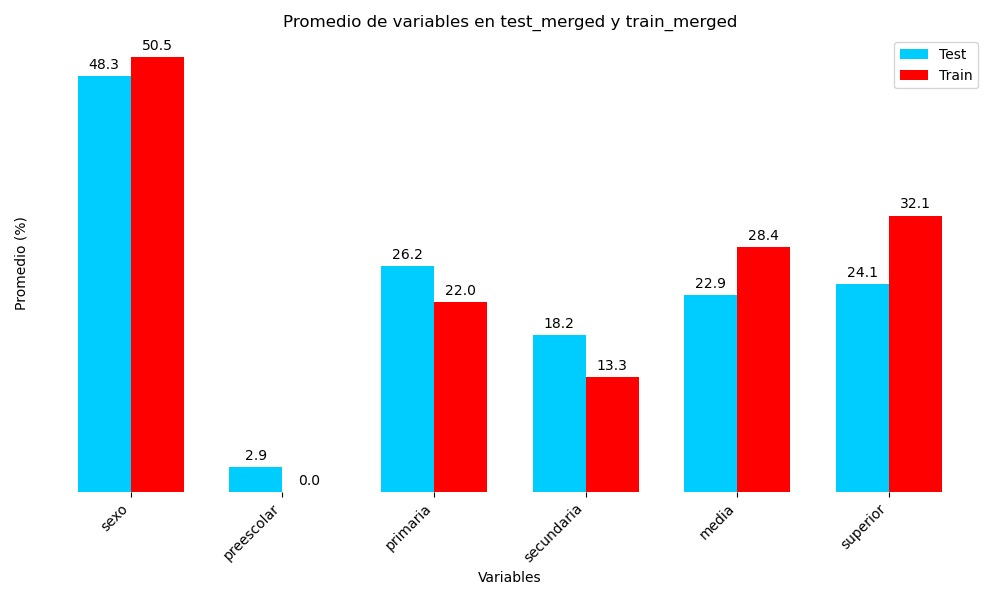
\includegraphics[width=16cm]{../Views/Grafico1.jpeg}
	\caption*{\small Fuente: Elaboración propia con base en datos de la GEIH }
\end{figure} 

Si bien ambas muestras no poseen los mismos valores promedios, se puede afirmar que no existe un patrón en la diferencias, es decir, no puede afirmarse, por ejemplo, que los individuos de la muestra de entrenamiento se encuentran más educados que la muestra de test. Como resultado, podemos decir que las muestras no se encuentran fuertemente desbalanceadas. La importancia de que las muestras se encuentren balanceadas radica en que permite confiar en la capacidad del modelo para generalizar y desempeñarse de manera robusta en datos nuevos.
El conjunto de prueba debe ser representativo de la misma distribución que el conjunto de entrenamiento, pero no debe tener datos duplicados de este. Esto asegura que la evaluación del modelo refleje su desempeño en escenarios del "mundo real", donde se enfrenta a nuevas observaciones.

\section{Modelos y Resultados}

En la presente sección se desarrollarán los distintos modelos predictivos de pobreza y se evaluarán y compararán sus desempeños. 

\subsection{Modelos}

Al momento de desarrollar modelos de predicción de pobreza, los mismos puede desarrollarse siguiendo dos enfoques; Por un lado, se encuentran los modelos de predicción de ingresos, en los cuales se los compara contra una línea de pobreza para clasificar a los hogares como pobres o no pobres en función de si se encuentran por debajo o por encima de ella. Por otro lado, se encuentran aquello modelos que tienen un enfoque dicotómico de clasificación, donde se evaluá la pobrabilidad de ser un hogar pobre o no, en función de distintas características individuales y del hogar. En el presente trabajo abordaremos ambos. 

\subsection*{Modelo 1}

El primer modelo que se explorará es el de una regresión lineal, donde se contemplan diversas características individuales que contribuyen a determinar el ingreso de un hogar y, en consecuencia, a la pobreza o no de los mismos. 

\[
\textit{y}= \beta_0 + \beta_1 \textit{Edad}  + \beta_2 \textit{Sexo} + \beta_3 \textit{Primaria} +\beta_4 \textit{Secundaria} +\beta_5 \textit{Media } + \beta_6 \textit{Superior } 
\]

La variable utilizada como dependendiente en esta regresión es la de \textit{Ingtot}, la cual reúne el ingreso total del hogar 

Este modelo presenta un muy elevado Mean Square Error (MSE) y un bajo $R^2$, con lo cual la capacidad predictiva de este modelo será bastante pobre. 

\subsection*{Modelo 2}

El segundo modelo a estimar también es el de una regresión lineal, pero donde ahora también se incorporan dummies indicativas para los beneficiarios de subsidios. Es probable que aquellos hogares que reciban asistencia social de algún tipo, posean una mayor probabilidad de encotrarse por debajo de la línea de pobreza. En particular se contemplan tres tipos de subdisidios: alimentación, transporte, familiar y educativo. 

\[
\begin{aligned}
\textit{y} = &\ \beta_0 + \beta_1 \textit{Edad} + \beta_2 \textit{Sexo} + \beta_3 \textit{Primaria} 
+ \beta_4 \textit{Secundaria} + \beta_5 \textit{Media} \\
& + \beta_6 \textit{Superior} + \beta_7 \textit{Subsidio\_alimentacion} 
+ \beta_8 \textit{Subsidio\_transporte} \\
& + \beta_9 \textit{Subsidio\_familiar} + \beta_{10} \textit{Subsidio\_educativo}.
\end{aligned}
\]



Si bien en esta instancia se logra reducir el $R^2$, en este caso,  el MSE continúa siendo muy elevado. 

\subsection*{Modelo 3}

Tal como se mencionó en el inicio de la presente sección, el problema de predicción de la pobreza podía realizarse a traves de un modelo selección o a partir de un modelo de predicción de ingresos. En este caso, abordaremos un modelo \textit{Logit} para predecir la probabilidad de que un hogar sea pobre, utilizando como variable dependiente a la variable \textit{pobre}, la cual toma valor uno en caso de que el hogar encuestado sea pobre y cero en caso contrario. 

La probabilidad de ser pobre $p_i $  se define como:

\[
p_i = \frac{e^{X_i \beta}}{1 + e^{X_i \beta}}
\]	

Siendo $X_i$ los distintos regresores que contribuyen a la probabilidad de ser pobre. En este caso, se optó por continuar con las mismas variables dicotómicas que se han utilizado anteriormente. Para este modelo se encuentra que la exactitud en el conjunto de entrenamiento es de 0.7068

\subsection*{Modelo 4}

Se utilizará en este caso el algoritmo de \textit{CARTs}  (Classification and Regression Trees). Los árboles de decisión pueden utilizarse para construir modelos de clasificación como de regresión. En esta oportunidad nos centraremos en los segundos. 

El primer modelo CARTS que se estimará es el siguiente: 

\[
\begin{aligned}
\textit{y} = &\ \beta_0  + \beta_1 \textit{Sexo} + \beta_2 \textit{Primaria} 
+ \beta_3 \textit{Secundaria} + \beta_4 \textit{Media}  + \beta_5 \textit{Superior} 
\end{aligned}
\]

Bajo esta nueva metología de entrenamiento de nuestro modelo se encuentra que la exactitud en el conjunto de entramiento continúa siendo 0.7068. Con lo cual, se puede afirmar que la nueva metodología no generó un impacto a la hora de mejorar la precisión de estimación. 


\subsection*{Modelo 5}

En esta oportunidad, continuamos utilizando un modelo bajo entrenamiento CARTs pero utilizando como variables independientes aquellas que corresponde a subsidios. En particular, el modelo que se estima es 

\[
\begin{aligned}
\textit{y} = &\ \beta_0 + \beta_1 \textit{Sexo} + \beta_2 \textit{Subsidio\_alimentacion} 
+ \beta_3 \textit{Subsidio\_transporte} \\
& + \beta_4 \textit{Subsidio\_familiar} + \beta_{5} \textit{Subsidio\_educativo}.
\end{aligned}
\]

Se puede observar el \textit{acurrancy score} se eleva a 0.7430, elevándose así su capacidad predictiva. 


\subsection*{Modelo 6}

Finalmente, se estima un modelo bajo metodología CARTs, donde se incluyen a todas las variables utilizadas hasta entonces. Esto es, se estima:

\[
\begin{aligned}
\textit{y} = &\ \beta_0  + \beta_1 \textit{Sexo} + \beta_2 \textit{Primaria} 
+ \beta_3 \textit{Secundaria} + \beta_4 \textit{Media} \\
& + \beta_5 \textit{Superior} + \beta_6 \textit{Subsidio\_alimentacion} 
+ \beta_7 \textit{Subsidio\_transporte} \\
& + \beta_8 \textit{Subsidio\_familiar} + \beta_{9} \textit{Subsidio\_educativo}.
\end{aligned}
\]

En esta oportunidad, se puede observar que la adición de más variables puede haber generado un sobreajuste en la muestra de entrenamiento, lo que ocasionó que el \textit{acurrancy score} disminuya  a 0.6477. Si bien el modelo puede tener un buen desempeño en el conjunto de entrenamiento, el rendimiento en el conjunto de prueba, medido a través de distintas métricas, tales como exactitud (accuracy), precisión, recall, F1-score, entre otra, puede ser muy bajo debido a la existencia de sobreajuste \textit(overfitting). Esto imposibilita que el modelo sea capaz de generalizar bien a datos nuevos. 


\subsection*{Modelo 7}

Como último algoritmo a utilizar para predecir pobreza, se evaluará la metodología de \textit{Random Forest}.  Esta estrategia es presentada como una extensión de los árboles de decisión que permite sobrepasar algunas de las limitaciones que poseen CARTs. Aunque CART es una metodología simple, interpretativa y efectiva en algunos casos, Random Forest ofrece mejoras significativas en términos de generalización, robustez y manejo de datos complejos. Estas ventajas hacen que Random Forest sea una opción más adecuada en la realidad, cuando existen datos con mucho ruido, alta dimensionalidad o clases desbalanceadas. 

Se estimará el siguiente modelo con dicha metodología: 

\[
\begin{aligned}
\textit{y} = &\ \beta_0  + \beta_1 \textit{Sexo} + \beta_2 \textit{Primaria} 
+ \beta_3 \textit{Secundaria} + \beta_4 \textit{Media}  + \beta_5 \textit{Superior} 
\end{aligned}
\]

La exactitud del conjunto de entrenamiento es de 0.7068, coincidente con modelos previamente estimados. 

\subsection*{Modelo 8}

Por último se estima la siguiente especificación bajo Random Forest 

\[
\begin{aligned}
\textit{y} = &\ \beta_0  + \beta_1 \textit{Sexo} + \beta_2 \textit{Primaria} 
+ \beta_3 \textit{Secundaria} + \beta_4 \textit{Media} \\
& + \beta_5 \textit{Superior} + \beta_6 \textit{Subsidio\_alimentacion} 
+ \beta_7 \textit{Subsidio\_transporte} \\
& + \beta_8 \textit{Subsidio\_familiar} + \beta_{9} \textit{Subsidio\_educativo}.
\end{aligned}
\]

Una vez más la adición de variables, no ha ayudado a mejorar la exactitud del conjunto de entramiento. 


\subsection{Resultados}

Los resultados obtenidos a lo largo de los distintas especificaciones de modelos y bajo la utilización de diversos algoritmos como lo fueron: Regresiones Lineales, Logit, CARTs y Random Forest, dan cuenta de cierta debilidad a la hora de predecir el nivel de pobreza. 

En este trabajo se ha encontrado que los modelos que mejor calificación han tenido para predecir el nivel de pobreza han sido los modelos de regresiones lineales. No obstante, no puede interpretarse ello como señal de que son estos los modelos que mejor desempeño poseen en un contexto generalizado. 

El presente análisis vislumbra ciertas debilidades.  En primer lugar, las variables elegidas como regresores en los distintos modelos pueden no haber sido las óptimas. En particular, nos centramos en características individuales para predecir pobreza a nivel hogar. No osbtante, variables relacionadas con la estructura del hogar y como este esté compuesto, pueden ser sumamente relevantes en la determinación de pobreza de un hogar.  Los hogares con menor cantidad de miembros capaces de ser empleados relativo a los dependientes, tal como un mayor porcentaje de niños, ancianos y otros individuos no aptos para trabajar, tienen menos flexibilidad. \footnote{Cazzaniga,F. y Sarmiento-Barbieri, I. 2010. Probabilidad de un Hogar de Permanecer en la Pobreza,Cuartas Jornadas de Jóvenes Investigadores UNT - CONICET}. De esta manera, incluir variables tales como cantidad de miembros en el hogar, proporción de niños, proporción de adultos mayores, entre otras, podrían haber mejorado nuestro análisis. 

En segundo lugar, los hiperparámetros utilizados para el desarrollo de las distintas metodologías, pueden no haber sido los óptimos. Un mayor detenimiento en la elección de los mismos, podría haber mejorado nuestras estimaciones sustancialmente. 


\section{Conclusiones}

El presente estudio ha evaluado el desempeño de distintos modelos predictivos para el pronóstico de la pobreza a nivel de hogar, basándose en datos obtenidos de la Gran Encuesta Integrada de Hogares (GEIH) de Bogotá en 2018. A través de la implementación y comparación de diversos enfoques de modelado, se ha evidenciado que las características demográficas, educativas y la influencia de políticas públicas son factores determinantes en la predicción de la pobreza.

A pesar de que los modelos de regresión lineal han mostrado un desempeño notable , es fundamental reconocer las limitaciones inherentes a la selección de variables y la optimización de hiperparámetros en los modelos de CARTs y Random Forest. La inclusión de variables adicionales, como la estructura del hogar y la proporción de miembros dependientes, podría enriquecer el análisis y mejorar la capacidad predictiva de los modelos.

Este trabajo predente dar una introducción a la construcción de modelos predictivos en un contexto donde las políticas públicas deben ser cada vez más eficientes y la capacidad de predecir la pobreza con mayor exactitud se convierte en una herramienta invaluable para maximizar el impacto de las estrategias implementadas. 

\end{document}